\documentclass[a4paper]{article}

\usepackage[spanish]{babel} %español
\usepackage[utf8]{inputenc} %tildes
\usepackage{amsmath}
\usepackage{graphicx} %imagenes
\usepackage{array} %tablas
\usepackage{caption}  
\usepackage{float} %fijar
\usepackage{wrapfig}
\usepackage{subcaption}
\usepackage{amsfonts}
\usepackage{amssymb}
\usepackage{multicol}
\usepackage{changepage}
\usepackage{cite}
\usepackage{url}
\usepackage{booktabs}
\usepackage{hyperref}
\usepackage{multirow}

\begin{document}	
	\begin{titlepage}
	\begin{center}
		\vspace*{-1in}
			
		\begin{figure}[tbh]
			\centering
			
\includegraphics[width=0.7\linewidth]{eafit}
			\label{fig:eafit}
		\end{figure}
			
			ESCUELA DE ECONOMÍA Y FINANZAS\\
			\vspace*{0.6in}
			
		\begin{large}
		    Abril 20 de 2021\\
		\end{large}
			\vspace*{0.2in}
			
		\begin{Large}
			\textbf{Brechas salariales de los docentes en Colombia} \\
		\end{Large}
			\vspace*{0.3in}
			
		\begin{large}
			César Enrique Herrera de la Hoz\\
			Julián Alberto Aléman Muñoz\\
			Juan Manuel Dominguez Cuentas\\
			Walter Alfredo Salas Zapata\\
			Juan Camilo Olaya Monsalve
		\end{large}
			\vspace*{0.3in}
			\rule{80mm}{0.1mm}\\
			\vspace*{0.1in}
			
		\begin{large}
			Revisor: \\
			Andrés Ramírez Hassan\\
		\end{large}  	
			
	\end{center}	    
	\end{titlepage}
	
\newpage
    \section{Introducción}
Un resultado central de García, Maldonado, Perry, Rodríguez \& Saavedra (2014) indica que si se toman dos escuelas de similar composición socioeconómica y desempeños diferentes en pruebas estandarizadas en Colombia, el único factor que parece explicar dicha diferencia es la calidad de los docentes (medida a través de las percepciones de los estudiantes). En otras palabras, el estudio muestra que los docentes son el factor escolar más importante para el aprendizaje de los estudiantes. Este resultado se relaciona con la literatura académica a nivel mundial que da un papel central al papel de los docentes en los procesos de aprendizaje. En este sentido, se puede aumentar el logro estudiantil con innovaciones de política educativa que mejoren los procesos de selección docente, así como su evaluación, formación y, como punto central para el presente taller de Econometría, su remuneración (García \textit{et al.}, 2014).

Referentes internacionales por el alto desempeño estudiantil como Finlandia, Singapur, Canadá (Ontario) y Corea del Sur, dan prioridad a potenciar de manera significativa el desarrollo de los docentes en la política educativa. Entre otras características, estos países tienen sistemas de formación universitaria docente de alta calidad, apuestan por la investigación y la práctica pedagógica y el ingreso a la profesión docente es competitivo y atractivo para los mejores bachilleres (García \textit{et al.}, 2014). En contraste, se pueden encontrar estudios que relacionan baja calidad académica y bajos incentivos a los docentes, como su remuneración. Así, Asadullah (2006) en Bangladesh demostró que los docentes tienen salarios más bajos que las personas no-docentes que tienen características similares (incluyendo aspectos de capital humano). Este estudio encontró que la brecha se mantiene, aun cuando la estimación se controla por sexo y ubicación (rural/urbano). De igual forma, Mizala \& Ñopo (2016) compararon la brecha salarial de los docentes de 14 países de América Latina y encontraron que los salarios de estos eran menores que los salarios de otras ocupaciones.

En Colombia, a diferencia de los países exitosos, la docencia en los niveles de preescolar, primaria y bachillerato, no atrae a los mejores bachilleres del país (García \textit{et al.}, 2014). Los docentes no encuentran grandes oportunidades de actualización acorde a las necesidades y no tienen una remuneración atractiva. Y según cálculos de García \textit{et al.} (2014), “cerca de la tercera parte de los docentes en primaria y de la cuarta parte de los docentes en secundaria no cuentan con formación universitaria profesional” (p. 24). A lo anterior se suma una complejidad adicional: las zonas más apartadas del país (generalmente con los mayores índices de pobreza o afectaciones por la violencia), son las que tienen una mayor proporción de profesores en estas condiciones.\\

En el presente trabajo se retoman los análisis presentados por García \textit{et al.} (2014). Establecemos una serie de observaciones técnicas y planteamos cuatro modelos para determinar la actual brecha salarial entre docentes y una serie de profesiones pertenecientes a ramas seleccionadas de la economía colombiana. A partir de nuestra metodología, se observa que varias de las recomendaciones realizadas por García \textit{et al.} (2014) mantienen validez para mejorar la remuneración docente.
    
%%%%%%%%%%%%%%%%%%%%%%%%%%%%%%%%%%%%%%%%%%%%%%%%%%%%%%%%%%%%%%%%%%%%%%%%%%%%%%%%%%%%%%%%%%%%%%%%%%%%   
    \section{Colombia: tras la excelencia docente y una mejor remuneración}
Dado el contexto colombiano, García \textit{et al.} (2014) realizan una evaluación integral a la situación docente. Revisan aspectos como la oferta de programas de actualización, la evaluación de desempeño, el mejoramiento permanente de los contenidos pedagógicos, la determinación de ascensos y promociones de los profesores que han ingresado bajo el Estatuto 1278\footnote{Decreto 1278 de junio 19 de 2002, “por el cual se expide el Estatuto de Profesionalización Docente”.} y la remuneración (aspecto central del presente Taller de Econometría). En este último aspecto los autores encuentran: i) que los docentes colombianos tienen ingresos 18\% menores con respecto a los profesionales de otras ocupaciones que atraen a los bachilleres con puntajes más altos en la Prueba Saber 11. Y ii), los salarios docentes tienen una baja varianza porque están definidos únicamente por el grado en el escalafón en que cada uno se encuentra. Adicionalmente, para los docentes el salario permanece relativamente constante durante la vida laboral. Lo anterior, concluyen los autores, impide cautivar y vincular a mejores candidatos a la docencia, y premiar el esfuerzo de los docentes actuales.

Teniendo en cuenta los dos hallazgos sobre la remuneración docente, García \textit{et al.} (2014) tienen dos propuestas: i) aumentar el salario mensual para los docentes regidos bajo el Estatuto 1278 para equipararlos a los salarios de las profesiones seleccionadas. De esta forma, indican los autores, se podría atraer a los individuos más capacitados a la carrera docente y empinar las curvas salariales, especialmente para docentes que obtengan maestrías (aumentar la varianza en los salarios para atraer personas sobresalientes a la profesión). Y ii), mejorar el sistema de incentivos monetarios y no monetarios, para que los docentes sobresalientes puedan alcanzar remuneraciones más altas (incentivos al desempeño).

Con respecto al aumento salarial, García \textit{et al.} (2014) proponen un incremento salarial para todos los docentes regidos por el Estatuto 1278. En especial, sugieren seguir el procedimiento aplicado a la nivelación salarial que ya se ha realizado a los docentes del Estatuto 1278 (en el 2008, 2009 y 2010). Adicionalmente, proponen la realización de estimaciones quinquenales para identificar en qué porcentaje aumentan los salarios promedio en las profesiones más competitivas y con los mejores profesionales, para asegurar siempre que la profesión docente tenga salarios competitivos en el mercado.

Con respecto a la baja varianza de los salarios docentes, proponen premiar a los docentes cuyos resultados laborales sean sobresalientes. Y plantean otorgar bonificaciones a: i) docentes con evaluaciones de desempeño en niveles superiores en las pruebas de ascenso que ya existen; ii) docentes que sean elegidos pares evaluadores; y iii), docentes en zonas de difícil acceso. Aunque este último aspecto ya existe en Colombia, García \textit{et al.} (2014) proponen mejorar la bonificación para ayudar, por ejemplo, a la adquisición de vivienda. Adicional a lo anterior, piden la creación de un concurso de becas condonables para que los docentes puedan realizar una maestría o un doctorado, y el beneficio a los docentes que trabajan en zonas de difícil acceso para que después de tres años puedan elegir un traslado a su lugar de preferencia.

A pesar de que los resultados y conclusiones de García \textit{et al.} (2014) son consistentes con la realidad de Colombia y otros países, tres aspectos se pueden constituir en limitaciones metodológicas

   \subsection{Análisis de cohortes}
Con el objetivo de analizar cómo cambia el ingreso a lo largo de la vida productiva, García \textit{et al.} (2014) “calcularon los salarios promedio por mes de los distintos grupos de trabajadores para cinco cohortes de edades diferentes: 20-29, 30-34, 35-44, 45-54 y 55-64 años de edad” (p. 167). Los datos con los que contaban los investigadores eran datos de sección cruzada de la GEIH de 2011, y con ese tipo de datos no se puede hacer este análisis.

Este tipo de análisis requiere datos longitudinales en los que las unidades de análisis -los docentes- son observadas en diferentes periodos de tiempo -salario en el año $Y_i$ -. Por esa razón, en este tipo de estudios los salarios se transforman a valores constantes. Estos dos rasgos son comunes en investigaciones que estudian cambios en el salario en el tiempo. Por ejemplo, los estudios de Lee \& Wolpin (2010) y Murnane, Singer \& Willett (1987), a pesar de ser estudios de épocas muy diferentes, investigan cambios salariales en el tiempo y para hacerlo tienen en cuenta estos dos rasgos: datos longitudinales y valores constantes. 

   \subsection{Ajuste de salarios por hora de trabajo}
García \textit{et al.} (2014) señalan que los docentes trabajan en promedio 12 horas menos que el grupo de comparación del estudio. Este dato lo proporcionan en las estadísticas descriptivas. Los investigadores pudieron evaluar si tales diferencias eran significativas y, en caso positivo, ajustar el modelo utilizando como variable dependiente el promedio del salario/hora en lugar del promedio del salario mensual. Ajustes de este tipo hicieron en otros estudios donde se compararon los salarios de los docentes con los de otros profesionales de similares características (Mizala \& Ñopo, 2016; Asadullah, 2006). En el estudio de brechas salariales de América Latina (Mizala \& Ñopo, 2016) se hicieron incluso las dos estimaciones (sin ajuste y con ajuste), y se observó que la brecha se redujo al hacer el ajuste del salario por horas.

   \subsection{Definición de los grupos de comparación}
García \textit{et al.} (2014) no distinguieron entre los docentes que pertenecen al estatuto de 1979 y los que pertenecen al Estatuto 1278. Esto significa que docentes que pertenecen a regímenes salariales diferentes quedaron en el mismo grupo y no se sabe qué efecto pudo tener la pertenencia a un estatuto determinado en la brecha salarial. Si se utilizan los datos de la GEIH 2019 tampoco se podrá hacer esa distinción, pero es probable que ahora se encuentren más docentes del estatuto de 2002 en comparación con la investigación que utilizó datos del 2011.
   
%%%%%%%%%%%%%%%%%%%%%%%%%%%%%%%%%%%%%%%%%%%%%%%%%%%%%%%%%%%%%%%%%%%%%%%%%%%%%%%%%%%%%%%%%%%%%%%%%%%%
    \section{Metodología}
Una vez analizadas las posibles limitaciones de García \textit{et al.} (2014), nuestro trabajo se centró en elegir unos datos y unos modelos para identificar las brechas salariales entre docentes y un grupo de profesiones seleccionadas. A continuación se presentan los detalles.

   \subsection{Datos}
En la encuesta GEIH 2019, los profesores fueron filtrados a partir de las ramas de actividad del CIIU 3 (2015): 8011, 8012, 8021 y 8022, excluyendo docentes de educación superior. Adicionalmente, excluimos aquellos profesores sin estudios profesionales o de postgrado ya que durante el régimen docente previo a 2002 los profesores no requerían estudios profesionales. Y se optó por tener un grupo de comparación construido a partir de 40 ramas de actividades profesionales que pueden constituirse en potenciales áreas llamativas para las personas por los salarios que se ofrecen (ver Anexo A). En el Cuadro 1 y Gráfico 1 se resumen unas características de la muestra.

\begin{table}[htbp]
	\centering
	\caption{Caracterización de los datos}
	\begin{tabular}{|clr|}
		\toprule
		\multicolumn{1}{|l}{\textbf{Caraterística}} & \textbf{Grupos} & \multicolumn{1}{l|}{\textbf{Totales}} \\
		\midrule
		\multirow{2}[4]{*}{\textbf{Sexo}} & Hombres & 56.875 \\
		\cmidrule{2-3}          & Mujeres & 70.253 \\
		\midrule
		\multicolumn{1}{|c}{\multirow{2}[4]{*}{\textbf{Grupos de comparación}}} & \multicolumn{1}{p{6.355em}}{Profesiones\newline{}seleccionadas} & 125.945 \\
		\cmidrule{2-3}          & Docentes & 1.183 \\
		\bottomrule
	\end{tabular}
    \caption*{Fuente: Elaboración propia}
	\label{tab:1}
\end{table}

\begin{figure}[htbp]
	\centering
	\caption{Histograma de las variables sociodemográficas}
	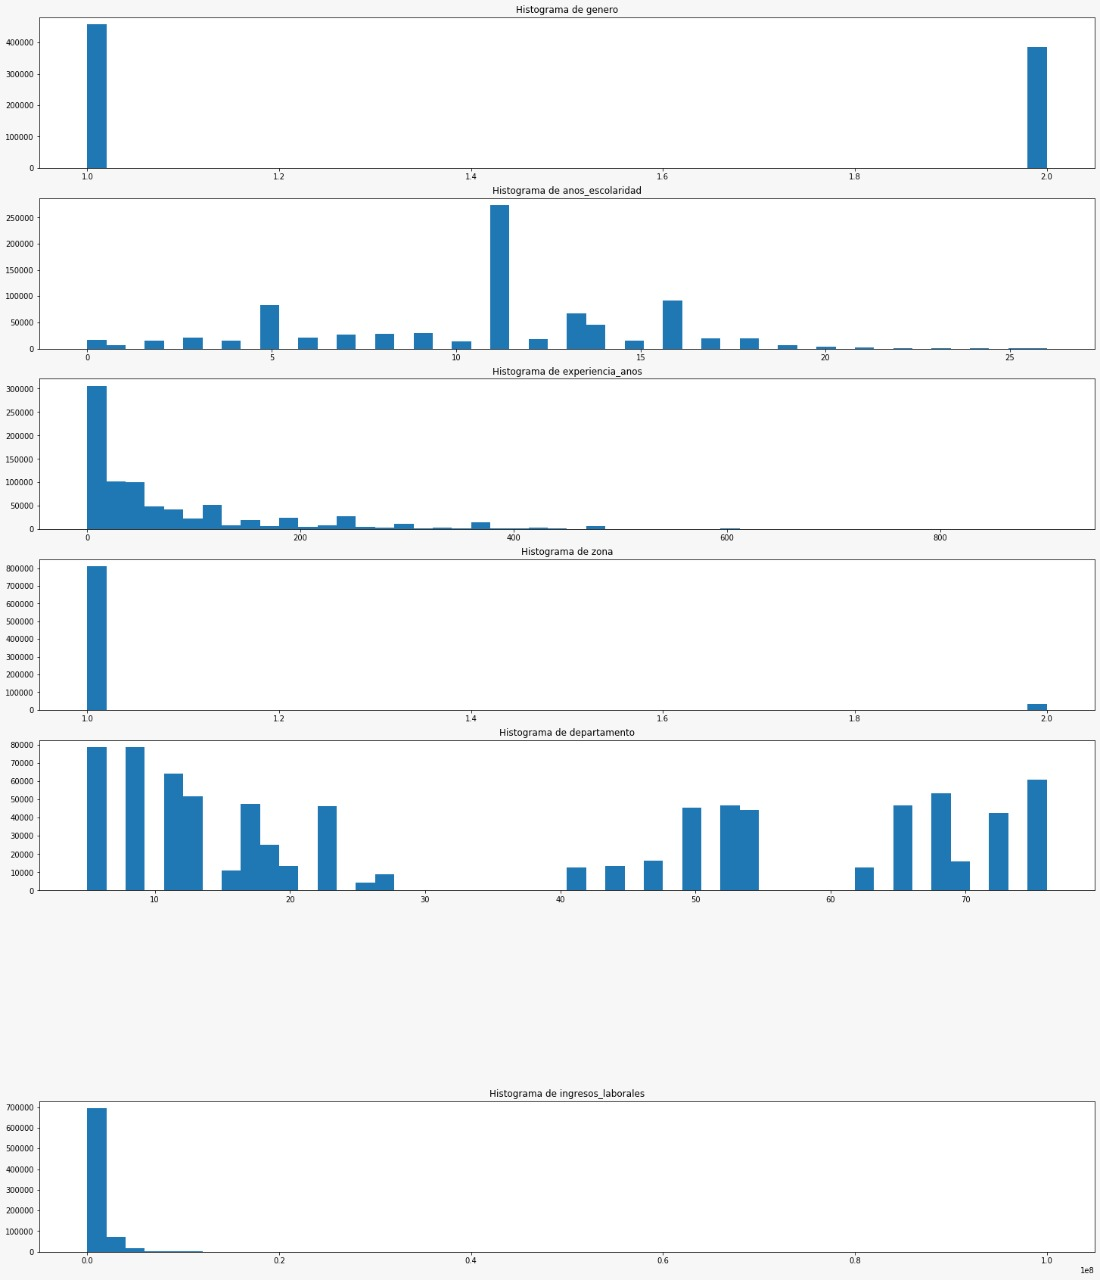
\includegraphics[width=1\linewidth, height=0.4\textheight]{fig1}
	\caption*{Fuente: Elaboración propia}
	\label{fig:fig1}
\end{figure}

   \subsection{Modelos y resultados}
\textbf{Modelo 1:} Se planteó un modelo siguiendo la metodología de García \textit{et al.} (2014), pero con el manejo de datos que proponemos para la GEIH 2019

\begin{equation}
log(W_{i})=X_{i}'\beta + \alpha PU_{i}+\varepsilon_{i}
\end{equation}
donde $W_i$ es el ingreso mensual, $X_{i}'$ es un vector de características socioeconómicas que incluye el género, el nivel educativo en años de escolaridad, la experiencia y la zona urbano/rural y departamento; y $PU_i$ es la variable dicotómica que captura si el entrevistado es un profesor o no. Con este modelo, se encontró una diferencia salarial del 22\% entre los docentes y las profesiones seleccionadas.\\

\textbf{Modelo 2:} Con el ánimo superar algunas de las limitaciones del estudio mencionadas anteriormente, se realizó un cambio en la variable ingresos: pasamos de salario mensual a salario/hora. Para esto propuso el siguiente modelo

\begin{equation}
log(S_{i})=X_{i}'\beta + \alpha PU_{i}+\varepsilon_{i}
\end{equation}
donde $S_i$ es el salario/hora. Una de las explicaciones a variación metodológica se encuentra en García \textit{et al.} (2014) que afirman que los profesores trabajan menos horas semanales que trabajadores de otras ocupaciones y profesiones seleccionadas. Se encontró una diferencia salarial del 15.99\% entre los docentes y las profesiones seleccionadas.\\

\textbf{Modelo 3:} La revisión bibliográfica nos permitió plantear un tercer modelo basado en la ecuación de Mincer. En particular, se optó por este tipo de modelo debido a que este enfoque surgió como una propuesta para analizar el perfil de ingresos de una persona a lo largo de su vida cuando solo se tienen datos de corte transversal (Galassi \& Andrada, 2009), como en el caso de la GEIH 2019. Este es el modelo

\begin{equation}
log(S_{i})=X_{i}'\beta + \alpha PU_{i}+\lambda_{1}Exp^{2}+\lambda_{2}Exp+\varepsilon_{i}
\end{equation}

En donde la variable $X_{i}'$ ya no incluye la experiencia. Con este modelo se encontró una diferencia salarial del 15.76\% entre los docentes y las profesiones seleccionadas.\\

\textbf{Modelo 4:} Dado que encontramos una brecha salarial muy parecida entre los modelos 2 y 3, se exploró una cuarta opción conservando el modelo 3, pero haciendo un ajuste en la muestra utilizando un algoritmo de comparación KNN. Este aplica una mejora a la selección de profesionales que consiste en obtener una distancia euclidiana entre las características de este grupo y el grupo de profesores. Esto permite seleccionar del grupo de profesionales a aquellos que tienen mayor afinidad en sus características con los docentes (esto es: años de escolaridad, experiencia en años y zona urbana o rural). Encontramos una diferencia salarial del 15,01\% entre los docentes y las profesiones seleccionadas.\\

El desempeño de los modelos se puede observar en el Cuadro 2, donde se calculan diferentes métricas para evaluar los modelos. Estas medidas comprenden AIC que permite calcular la pérdida de información del modelo, medidas de bondad de ajuste ($R^2$ y $R^2$ ajustado), y la 	distancia media cuadrática mínima que es una medida de precisión para comparar errores de pronóstico.

\begin{table}[htbp]
	\centering
	\caption{Métricas de decisión para seleccionar el modelo}
	\begin{tabular}{|l|r|r|r|r|}
		\toprule
		\textbf{Métricas de decisión} & \multicolumn{1}{l|}{\textbf{Modelo 1}} & \multicolumn{1}{l|}{\textbf{Modelo 2}} & \multicolumn{1}{l|}{\textbf{Modelo 3}} & \multicolumn{1}{l|}{\textbf{Modelo 4}} \\
		\midrule
		AIC   & 288195.6 & 280916.7 & 280294.1 & 4123.4 \\
		$R^2$    & 0.1685 & 0.1846 & 0.1886 & 0.275 \\
		$R^2$ ajustado & 0.1685 & 0.1846 & 0.1886 & 0.2731 \\
		RMSD  & 14.4753 & 9.3713 & 9.3715 & 9.1811 \\
		\bottomrule
	\end{tabular}
	\caption*{Fuente: Elaboración propia}
	\label{tab:metricas}
\end{table} 

Es fácil notar que el Modelo 4 posee mejor rendimiento en todas la métricas usadas, mostrando que mejor capacidad de ajuste a la muestra debido a que su pérdida de información es menor y explica la proporción de variación de los resultados que puede explicarse por el modelo.

%%%%%%%%%%%%%%%%%%%%%%%%%%%%%%%%%%%%%%%%%%%%%%%%%%%%%%%%%%%%%%%%%%%%%%%%%%%%%%%%%%%%%%%%%%%%%%%%%%%%
    \section{Consideraciones finales}
Primero, los coeficientes de los cuatro modelos que planteamos en nuestro ejercicio coinciden en reafirmar la brecha existente entre los salarios de los docentes y las profesiones seleccionadas, en contra de los profesores. Con los datos del GEIH 2019, nuestro modelo 1 incluso muestra una brecha mayor a la encontrada por García et al. (2014).

Segundo, cuando los salarios se ajustaron por salario/hora, la brecha salarial pasó de 22\% a 15,99\%. Y una reducción parecida se encontró cuando se agregó el control experiencia, al pasar de 22\% a 15,76\%. Esto está relacionado con las menores horas semanales trabajadas por los docentes en comparación con los profesionales de las ramas seleccionadas.

Tercero, al utilizar el algoritmo KKN se corrige parte de la arbitrariedad que puede existir al seleccionar el grupo de profesiones de control. Con este método, en el modelo 4 la brecha salarial pasó de 22\% a 15,01\%, parecido a los modelos 2 y 3. Además, el modelo 4 mejoró la capacidad explicativa con un ajuste del 27,5\% en el $R^2$. 

Teniendo en cuenta los tres resultados anteriores, se plantea como recomendación mantener una política educativa enfocada al mejoramiento de las condiciones salariales de los docentes como una estrategia para llegar a altos estándares de calidad educativa, en concordancia con lo planteado por García et al. (2014) y otras experiencias internacionales. Dado este contexto, se pueden retomar las propuestas de García et al. (2014) para reducir los problemas relacionados con la brecha salarial entre docentes y otros profesionales: i) aumentar el salario mensual para los docentes regidos bajo el Estatuto 1278 para equipararlos a los salarios de las profesiones seleccionadas. Y ii), mejorar el sistema de incentivos monetarios y no monetarios, para que los docentes sobresalientes puedan alcanzar remuneraciones más altas. 

Las anteriores estrategias podrían atraer a los individuos más capacitados a la carrera docente y empinar las curvas salariales. Sin embargo, cabe mencionar que un excelente incentivo salarial no es la única motivación para que una persona decida convertirse en docente. Esta es una tarea integral que también incluye aspectos como el mejoramiento de la oferta de programas de actualización, la evaluación del desempeño, el ajuste permanente de los contenidos pedagógicos, la determinación de ascensos y promociones de los profesores, e incluso, un mayor reconocimiento social.

%%%%%%%%%%%%%%%%%%%%%%%%%%%%%%%%%%%%%%%%%%%%%%%%%%%%%%%%%%%%%%%%%%%%%%%%%%%%%%%%%%%%%%%%%%%%%%%%%%%%
\newpage
\thebibliography{9}
    \item Asadullah, N. (2006). Pay differences between teachers and other occupations: Some empirical evidence from Bangladesh. \textit{Journal of Asian Economics}, 17: 1044–1065. 
    
    \item Anderson, K., \& Esenaliev D. (2019). Gender Earnings Inequality and Wage Policy: Teachers, Health Care, and Social Workers in Central Asia. \textit{Comparative Economic Studies}, 61: 551–575.  \href{<url>}{https://doi.org/10.1057/s41294-019-00103-1}
    
    \item Galassi, G. \& Andrada, M.J. (2009). La relación entre educación e ingresos: ecuaciones de Mincer por regiones geográficas de Argentina. \textit{Jornadas Argentinas de Estudios de Población. Asociación de Estudios de Población de la Argentina}, San Fernando del Valle de Catamarca.
    
    \item García, S., Maldonado, D., Perry, G., Rodríguez, \& C., Saavedra, J. (2014). Tras la excelencia docente: Cómo mejorar la calidad de la educación para todos los colombianos. Bogotá: \textit{Fundación Compartir}.
    
    \item Lee, D. \& Wolpin, K. (2010). Accounting for wage and employment changes in the US from 1968–2000: A dynamic model of labor market equilibrium. \textit{Journal of Econometrics}, 156: 68–85.
    
    \item Mizala, A. \& Ñopo, H. (2016). Measuring the relative pay of school teachers in Latin America 1997–2007. \textit{International Journal of Educational Development}, 47: 20–32.
    
    \item Murnane, R., Singer, J. \& Willett, J. (1987). Changes in teacher salaries during the 1970s: The role of school district demographics. \textit{Economics of Education Review}, 6(4): 379-388.
    
    \item Base de datos: Departamento Administrativo Nacional de Estadística [DANE]. Gran Encuesta Integrada de Hogares 2019 [GEIH, 2019].
    

%%%%%%%%%%%%%%%%%%%%%%%%%%%%%%%%%%%%%%%%%%%%%%%%%%%%%%%%%%%%%%%%%%%%%%%%%%%%%%%%%%%%%%%%%%%%%%%%%%%%
\newpage
\appendix
    \section{Clases seleccionadas}
\begin{table}[H]
	\caption{Clases de profesiones selecionadas}
	\begin{tabular}{|rl|}
		\toprule
		6421  & Servicios telefónicos \\
		6422  & Servicios de transmisión de datos a través de redes \\
		6423  & Servicios de transmisión de programas de radio y televisión \\
		6424  & Servicios de transmisión por cable \\
		6511  & Banca central \\
		6512  & Actividades de los bancos diferentes del banco central \\
		6513  & Actividades de las corporaciones de ahorro y vivienda \\
		6514  & Actividades de las corporaciones financieras \\
		6515  & Actividades de las compañías de financiamiento comercial \\
		6519  & Otros tipos de intermediación monetaria n.c.p. \\
		6591  & Arrendamiento financiero (Leasing)  \\
		6592  & Actividades de las sociedades de fiducia \\
		6593  & Actividades de las cooperativas financieras y fondos de empleados \\
		6594  & Actividades de las sociedades de capitalización \\
		6595  & Actividades de compra de cartera (factoring) \\
		6596  & Otros tipos de crédito \\
		6599  & Otros tipos de intermediación financiera n.c.p. \\
		6601  & Planes de seguros generales \\
		6602  & Planes de seguros de vida \\
		6603  & Planes de reaseguros \\
		6604  & Planes de pensiones y cesantías \\
		6711  & Administración de mercados financieros \\
		6712  & Actividades de las bolsas de valores \\
		6713  & Actividades de comisionistas y corredores de valores \\
		6714  & Otras actividades relacionadas con el mercado de valores \\
		6715  & Actividades de las casas de cambio \\
		6716  & Actividades de los profesionales de compra y venta de divisas \\
		6719  & Actividades auxiliares de la intermediación financiera n.c.p. \\
		6721  & Actividades auxiliares de los seguros \\
		6722  & Actividades auxiliares de los fondos de pensiones y cesantías \\
		7210  & Consultores en equipo de informática  \\
		7220  & Consultores en programas de informática y suministro de programas de informática \\
		7230  & Procesamiento de datos \\
		7240  & Actividades relacionadas con bases de datos \\
		7250  & Mantenimiento y reparación de maquinaria de oficina, contabilidad e informática \\
		7290  & Otras actividades de informática \\
		7310  & Investigación y desarrollo experimental en el campo de las ciencias naturales y la ingeniería  \\
		7320  & Investigación y desarrollo experimental en el campo de las ciencias sociales y las humanidades  \\
		7421  & Actividades de arquitectura e ingeniería y actividades conexas de asesoramiento técnico \\
		7422  & Ensayos y análisis técnicos \\
		\bottomrule
	\end{tabular}
    \caption*{Fuente: Elaboración propia}
	\label{tab:profesiones}
\end{table}  

\end{document}



